\documentclass[
12pt,
a4paper,
pdftex,
czech,
titlepage
]{article}

\usepackage[a4paper, total={6in, 9in}]{geometry}
\usepackage[czech]{babel}
\usepackage[utf8]{inputenc}
\usepackage{lmodern}
\usepackage{textcomp}
\usepackage[T1]{fontenc}
\usepackage{amsfonts}
\usepackage{titlesec}
\usepackage{float}
\usepackage{calc}  
\usepackage{hyperref}
\usepackage{enumitem}  
\usepackage{graphicx}
\usepackage{fancyvrb}
\newcommand{\latex}{\LaTeX\xspace}
\newcommand{\tex}{\TeX\xspace}

\titleformat{\chapter}
  {\normalfont\LARGE\bfseries}{\thechapter}{1em}{}
\titlespacing*{\chapter}{0pt}{0ex plus 1ex minus .2ex}{2.0ex plus .2ex}

\begin{document}

\begin{titlepage}
	\vspace*{-2cm}
	{\centering
\includegraphics[scale=1.0]{logo.pdf}\par}
	\centering
	\vspace*{2cm}
	{\Large Semestrální práce z KIV/DBM2\par}
	\vspace{1.5cm}
	{\Huge\bfseries SPARQL Tool\par}
	\vspace{2cm}

	{\Large Martin Matas\par}
	{\Large A18N0095P\par}
	{\Large martinm@students.zcu.cz\par}

	\vfill

	{\Large \today}
\end{titlepage}

\tableofcontents
\thispagestyle{empty}
\clearpage

\section{Zadání}
\setcounter{page}{1}

Vytvořit Javascriptový nástroj, který bude snadno vložitelný do jiných
webových projektů (ideálně jeden javascript soubor k načtení v html
hlavičce) a bude umět:

\begin{itemize}
\item
  odeslat SPARQL dotaz na zadaný libovolný SPARQL endpoint (ajax)
\item
  vypsat výsledek dotazu do triviální webové tabulky
\item
  načíst/uložit dotaz do místní paměti problížeče (browser local
  storage)
\item
  spravovat uložené dotazy
\item
  vyhledávat v uložených dotazech
\item
  verzovat dotazy
\end{itemize}

\hypertarget{data}{%
\subsection{Data:}\label{data}}

\begin{itemize}
\item
  dle svého uvážení, případně na vyžádání dodám SPARQL datazy a
  příslušné datasety
\end{itemize}

\section{Řešení}

Nástroj byl po zvážení vypracován pomocí jazyka \texttt{TypeScript}, který umožňuje přeložení zdrojového kódu do Javascriptu ve standardu ECMAScript 5 (ES5). Standard ES5 byl zvolen předevší pro svoji rozšířenost, protože v dnešní době je podporován většinou prohlížečů a knihoven. Další nespornou výhodou jazyka TypeScript byla možnost napsat nástroj s využitím typové kontroly a možností OOP programování, díky čemuž je kód snadno pochopitelný a přehledný. \\

Pro správu závislostí a sestavení projektu byl využit nástroj \texttt{npm}, který se velmi často využívá ve spojení s klientskými aplikacemi. Pomocí tohoto nástroje byl založen projekt, nadefinovány potřebné závislosti pro vývoj a především skripty, které slouží k sestavení projektu a vygenerování dokumentace kódu. Zprovoznění projektu je poté velmi jednoduché, stačí mít pouze nainstalovaný nástroj \texttt{npm} a následně sestavit projekt jedním příkazem.

\subsection{Struktura aplikace}
\label{sec:structure}

Popis jednotlivých tříd a jejich využití je podrobně rozepsáno v přiložené dokumentaci v adresáři \texttt{docs/}.

\subsection{Struktura úložiště}

Aby bylo možné efektivně pracovat s dotazy uloženými v lokálním úložišti prohlížeče (localstorage), byla vytvořena jednoduchá interní struktura viz zdrojový kód níže. 

\begin{Verbatim}[samepage=true]
{
  queries: [						
    {
      name: string,
      queryString: Array<string>,
      currentVersion: number
    }
  ]
}
\end{Verbatim}

Každý dotazy typu \texttt{Query} je uložen uvnitř pole \texttt{queries}. Aby bylo možné dotazy verzovat, každý dotaz obsahuje pole všech verzí dotazu \texttt{queryString} a ukazatel definující aktuální verzi \texttt{currentVersion}.

\section{Uživatelská dokumentace}

\begin{figure}[h]
	\centering
	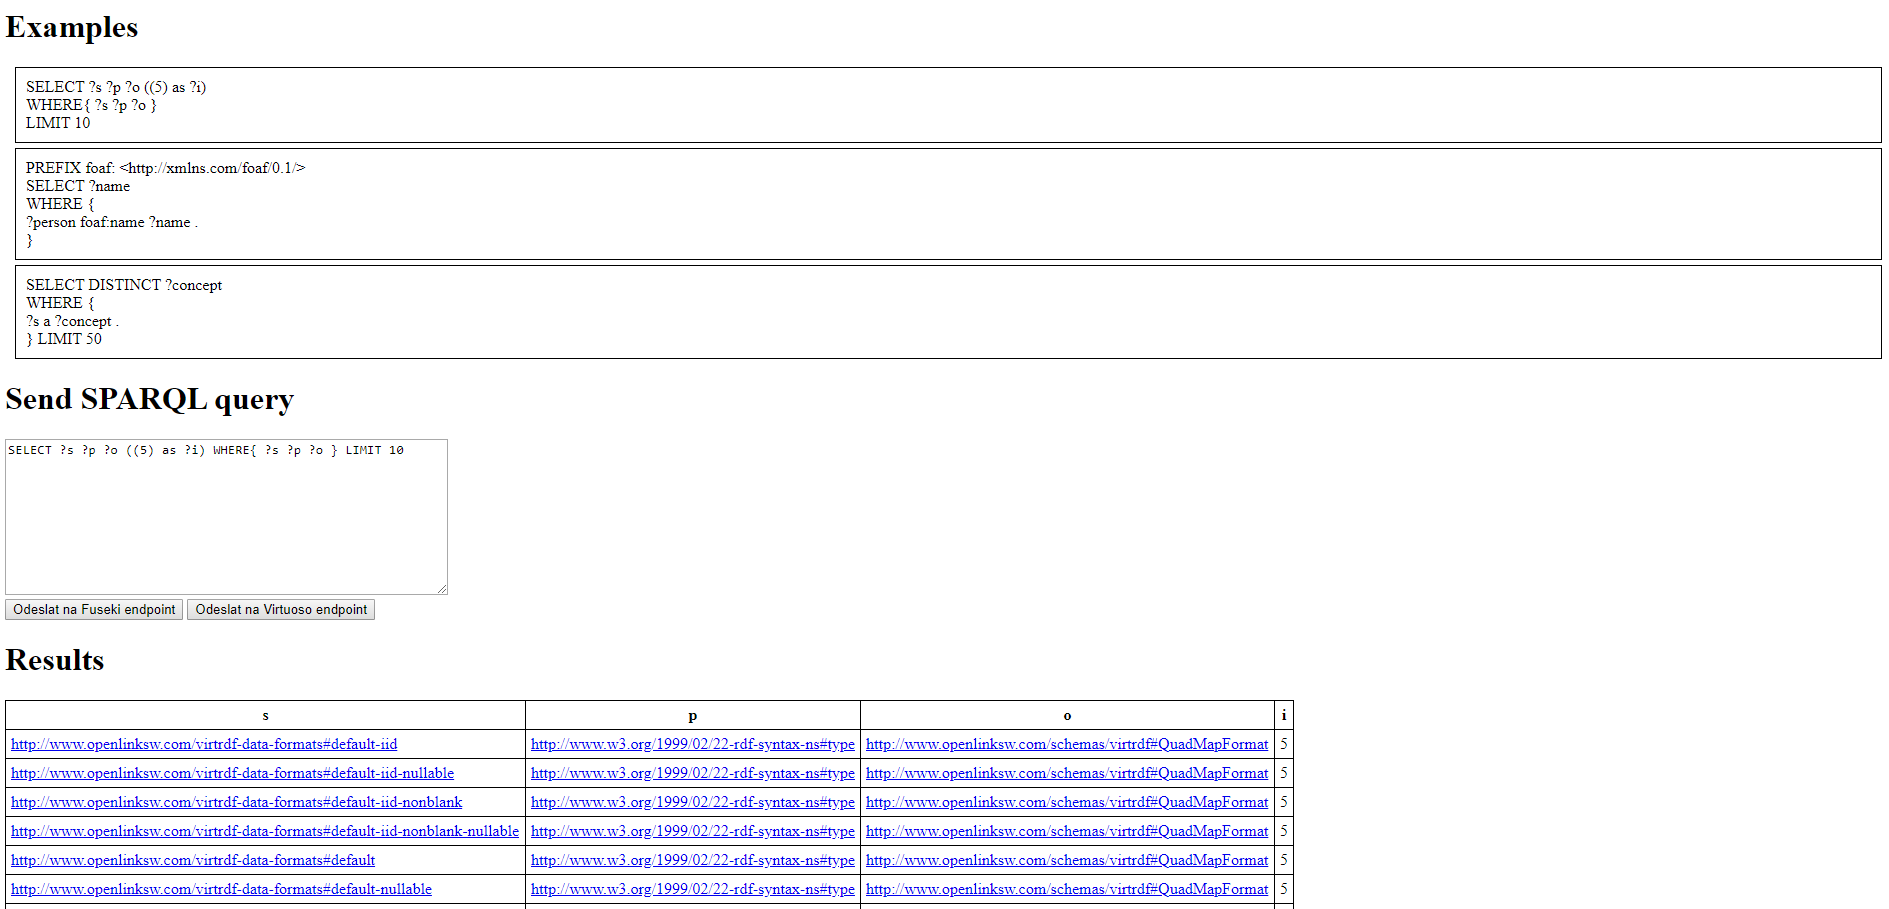
\includegraphics[width=\textwidth]{view}
	\caption{Ukázka UI aplikace.}
	\label{fig:ui}
\end{figure}

\subsection{Sestavení}
\label{sec:build}

Nástroj obsahuje již přeložené zdrojové kódy a vygenerovanou dokumentaci, ale v případě potřeby (např. při změně zdrojového kódu knihovny) lze projekt sestavit pomocí nástroje \texttt{npm}, který má definováno několik skriptů:

\begin{description}
    \item[clean] - vyčištění projektu od přeložených souborů a generované dokumentace
    \item[tsc] - přeložení knihovny
    \item[minify] - minifikace a znečitelnění zrojových souborů
    \item[docs] - vygenerování dokumentace kódu
    \item[build] - sestavení projektu
    \item[build:min] - sestavení projektu + minifikace a znečitelnění zrojových souborů
\end{description}

\noindent Jednotlivé skripty se spustí příkazem:

\begin{verbatim}
... \> npm run název_skriptu
\end{verbatim}

\subsection{Spuštění}

Program je možné spustit pomocí souboru \texttt{index.html}, který se nachází v kořenovém adresáři projektu. Nicméně je nejlepší si program sestavit (viz sekce \ref{sec:build}) pro ujištění se, že je skutečně použita aktuální verze nástroje. \\

Po otevření \texttt{index.html} se zobrazí webová stránky viz obrázek \ref{fig:ui}. V horní části jsou připraveny 3 ukázkové dotazy, které je možné spustit. Spuštění se provede kliknutím na jeden z dotazů a následným odesláním dotazu pomocí jednoho z tlačítek pod formulářem. Pro \texttt{Fuseki} endpoint je potřeba mít lokálně spuštěný daný server. V případě endpointu \texttt{Virtuoso} se jedná o server třetí strany, který by měl být dostupný, takže odpověď na daný dotaz by se měla zobrazit během okamžiku ve spodní sekci \texttt{Results} jako je tomu v ukázce na výše zmíněném obrázku.

V případě, že by server nefungoval nebo se odpověď nezobrazila, pravděpodobně mohla být chyba v dotazu. V tomto případě bude chyba vypsána v konzoli.\\

Může dojít k situaci kdy nástroj nebude fungovat, typicky tento problém nastával v prohlížeči IE11. Důvodem byl problém s lokálním úložištěm, které nefungovalo správně při spuštění stránky přímo z projektu. Pro správnou funkčnost bylo potřeba umístit \texttt{index.html} s adresářem \texttt{dist/} na lokální server (např. Apache) a tam stránku otevřít.

\subsection{Práce s knihovnou}

Popis práce s knihovnou a klíčovými třídami je podrobně popsán v souboru \texttt{README.md}.

\subsubsection{Modifikace knihovny}

Pokud by bylo potřeba knihovnu nějakým způsobem upravit, všechny změny je potřeba provést v souboru \texttt{src/sparqljs.ts} a následně nástroj sestavit viz sekce \ref{sec:build}.\\

Pokud by tedy například bylo potřeba upravit objekt \texttt{Query}, stačí nalézt příslušnou třídu a tu modifikovat. V případě této třídy bude ale potřeba také upravit formát JSON objektu, který přijímá konstruktor třídy \texttt{QueryList}. Konstruktor této třída totiž zpracovává předaný JSON objekt z lokálního úložiště a převádí jej na interní struktury a pravděpodobně by došlo při sestavení k chybě kvůli neodpovídající struktuře objektu na vstupu do konstruktoru. \\

V každém případě je doporučeno nejprve nastudovat přiloženou dokumentaci, kterou lze otevřít v prohlížeči souborem \texttt{docs/index.html}. Pokud dokumentace neexistuje, je možné ji vygenerovat viz sekce \ref{sec:build}. 

\subsubsection{Nasazení}

Pro nasazení aplikace do provozního prostředí je potřeba (v případě ukázkové aplikace) zkopírovat \texttt{index.html} s adresářem \texttt{dist/} na daný server. Pro tento případ je možné sestavit nástroj pomocí skriptu \texttt{build:min}, který sestaví projekt, minifikuje kód a znečitelní zdrojový kód knihovny.

\section{Závěr}

Nástroj splňuje požadavky zadání a je kompatibilní se všemi prohlížeči. Při implementaci jsem nenarazil na žádný problém. Problémy nastaly až při sestavení projektu, kdy nebylo jednoduché nastavit konfigurace tak, aby se generoval jeden soběstačný JS soubor.

\end{document}